\documentclass{article}


% if you need to pass options to natbib, use, e.g.:
%     \PassOptionsToPackage{numbers, compress}{natbib}
% before loading neurips_2023


% ready for submission
% \usepackage{neurips_2023}


% to compile a preprint version, e.g., for submission to arXiv, add add the
% [preprint] option:
    % \usepackage[preprint]{neurips_2023}


% to compile a camera-ready version, add the [final] option, e.g.:
\usepackage[final]{neurips_2023}


% to avoid loading the natbib package, add option nonatbib:
%    \usepackage[nonatbib]{neurips_2023}
% \usepackage[natbib]{neurips_2023}

\usepackage[utf8]{inputenc} % allow utf-8 input
\usepackage[T1]{fontenc}    % use 8-bit T1 fonts
\usepackage[hidelinks]{hyperref}       % hyperlinks
\usepackage{url}            % simple URL typesetting
\usepackage{booktabs}       % professional-quality tables
\usepackage{amsfonts}       % blackboard math symbols
\usepackage{nicefrac}       % compact symbols for 1/2, etc.
\usepackage{microtype}      % microtypography
\usepackage{xcolor}         % colors
\usepackage{adjustbox}
\usepackage{multirow}
\usepackage{graphicx}
\usepackage{pgfplots} 
    \usepgfplotslibrary{groupplots}
\usepackage{siunitx}
\usepackage{wrapfig}
\usepackage{booktabs}
\usepackage{pifont}
\usepackage{algorithm}
\usepackage{algpseudocode}
\usepackage{enumitem}
\usetikzlibrary{patterns}
\usepackage{amsmath, amssymb}
\usepackage{cleveref}
\usepackage{subcaption}
\usepackage{caption}
\usepackage{setspace}
% defined command
\newcommand{\comment}[1]{[\textcolor{red}{#1}]}
\newcommand{\cmark}{\ding{51}}%
\newcommand{\xmark}{\ding{55}}%
\renewcommand{\algorithmicrequire}{\textbf{Input:}}

%%%%%%%%% recover this if we want to do iclr format
% \def\setstretch#1{\renewcommand{\baselinestretch}{#1}}
% \setstretch{0.97}
% \addtolength{\parskip}{-1pt}
\usepackage[compact]{titlesec}
\titlespacing{\subsection}{0pt}{*1}{*0}
\setcitestyle{square}
\setcitestyle{citesep={,}}
%%%%%%%%%%%%%%%%%%%%%%%%%%%%%%%%%%%%%%%%%%%%%%%%%%%%%


\title{Efficiently Adapting Pretrained Language Models to New Languages}
% \title{Tool Manipulation with Open-source Large Language Models}


% The \author macro works with any number of authors. There are two commands
% used to separate the names and addresses of multiple authors: \And and \AND.
%
% Using \And between authors leaves it to LaTeX to determine where to break the
% lines. Using \AND forces a line break at that point. So, if LaTeX puts 3 of 4
% authors names on the first line, and the last on the second line, try using
% \AND instead of \And before the third author name.

\author{%
  Zoltan Csaki, Pian Pawakapan, Urmish Thakker, Qiantong Xu \\
  SambaNova Systems, Inc. \\
  Palo Alto, CA, USA \\
  \texttt{zoltan.csaki@sambanovasystems.com} \\
  % \texttt{\{qiantong.xu,fenglu.hong,bo.li,changran.hu,edison.chen,jian.zhang\}@sambanovasystems.com} \\
  % examples of more authors
  % \And
  % Coauthor \\
  % Affiliation \\
  % Address \\
  % \texttt{email} \\
  % \AND
  % Coauthor \\
  % Affiliation \\
  % Address \\
  % \texttt{email} \\
  % \And
  % Coauthor \\
  % Affiliation \\
  % Address \\
  % \texttt{email} \\
  % \And
  % Coauthor \\
  % Affiliation \\
  % Address \\
  % \texttt{email} \\
}

\begin{document}

\maketitle

\vspace{-1.5em}
\begin{abstract}

% State-of-the-art large language models are predominantly trained on English text and exhibit sub-optimal performance on other language, especially low resource languages such as Hungarian and Thai. 
% Pretraining a monolingual LLM from scratch requires a vast amount of text available in the language, but most languages do not have this amount of text available. 
% One way to mitigate that is to train a multi-lingual model, where low resource languages are trained with high resource languages. However, this requires a large amount of compute.
% In this paper introduce we introduce an approach to adapt an existing LLM pretrained on primarily English text to a new language that the model was not trained on. This paper shows how to adapt the tokenizer to have good fertility on the new language, the best way to mix the original language and the low resource language to maximize language transfer, and explores instruction tuning the model with a minimal amount of data in the low-resource language. 

Recent large language models (LLM) exhibit sub-optimal performance on low-resource languages, as the training data of these models is usually dominated by English and other high-resource languages. 
Furthermore, it is challenging to train models for low-resource languages, especially from scratch, due to a lack of high quality training data. 
Adapting pretrained LLMs reduces the need for data in the new language while also providing cross lingual transfer capabilities. However, naively adapting to new languages leads to catastrophic forgetting and poor tokenizer efficiency.
In this work, we study how to efficiently adapt any existing pretrained LLM to a new language without running into these issues.
In particular, we improve the encoding efficiency of the tokenizer by adding new tokens from the target language and study the data mixing recipe to mitigate forgetting.
Our experiments on adapting an English LLM to Hungarian and Thai show that our recipe can reach better performance than open source models on the target language, with minimal regressions on English. 


\end{abstract}

% \vspace{-0.5em}
\section{Introduction \& Related work}
% \vspace{-0.25em}
\label{sec:intro}
\section{Introduction}\label{sec:intro}
% Multi-armed bandit (MAB) is a classic sequential decision making problem \citep{auer2002finite}, where a learning agent chooses among competing actions sequentially to maximize its accumulative reward over time. 
% %Despite its simplicity, MAB exemplifies the exploration-and-exploitation dilemma that also exists in more complicated problems. 
% An important extension of MAB, named linear contextual bandit \citep{li2010contextual}, incorporates contextual information in the problem setting, by assuming a linear mapping between the context and expected reward. It has gained popularity in various applications, such as recommender systems \citep{li2010contextual}, display advertisement \citep{li2010exploitation} and clinical trials \citep{durand2018contextual}.
% Most existing linear bandit solutions are designed under a centralized learning setting, i.e., data is readily available at a central server. However, with the increasing public concerns of privacy, especially the bandit algorithms usually directly learn from user data,
% %more and more people are reluctant to provide their own data and strict regulations on data usage like GDPR have also went into effect \cite{voigt2017eu}, which makes 
% there is a growing demand to keep data decentralized and push the learning of bandit models to the client side. 
% % This idea is also made much more feasible due to the growing computational power of edge devices nowadays. 

% Federated learning has recently emerged as a promising setting for decentralized machine learning.
% % , and its effectiveness was first validated at a large scale by training a global model across all mobile devices via the Google Keyboard Android application \cite{konevcny2016federated}. 
% %The term ``federated learning" was first introduced by \citet{mcmahan2017communication} with an emphasis on efficiently training deep models over mobile device applications. As significant amount of later works have applied federated learning to other applications, there may be variations in its meaning for different research communities. 
% Since its debut in \citet{mcmahan2017communication}, there have been variations in its definition for different applications \citep{yang2019federated}.
% In this paper, we follow the general definition by \citet{kairouz2019advances}: multiple clients collaborate in solving a machine learning problem under the coordination of a central server, while keeping each client's raw data local. 
% So far, most existing works in federated learning study offline supervised learning problems \citep{konevcny2016federated,zhao2018federated}, where labeled training instances already sit on the client side. How to perform bandit learning under the federated learning setting remains underexplored.
As a popular online learning problem, linear contextual bandit has been used for a variety of applications, including recommender systems \citep{li2010contextual}, display advertisement \citep{li2010exploitation} and clinical trials \citep{durand2018contextual}. While most existing solutions are designed under a centralized setting (i.e., data is readily available at a central server), in response to the increasing application scale and public concerns of privacy, there is a growing demand to keep data decentralized and push the learning of bandit models to the client side.
% As a classic sequential decision making problem, linear contextual bandit has been widely used for a variety of real-world applications, including recommender systems \citep{li2010contextual}, display advertisement \citep{li2010exploitation} and clinical trials \citep{durand2018contextual}. 
% Most existing solutions are designed under a centralized learning setting, i.e., data is readily available at a central server. However, with the increasing public concerns of privacy, especially the bandit algorithms usually directly learn from user data,
% there is a growing demand to keep data decentralized and push the learning of bandit models to the client side. 
Federated learning has recently emerged as a promising setting for decentralized machine learning \citep{konevcny2016federated}.
% , and its effectiveness was first validated at a large scale by training a global model across all mobile devices via the Google Keyboard Android application \cite{konevcny2016federated}. 
%The term ``federated learning" was first introduced by \citet{mcmahan2017communication} with an emphasis on efficiently training deep models over mobile device applications. As significant amount of later works have applied federated learning to other applications, there may be variations in its meaning for different research communities. 
Since its debut in \citeyear{mcmahan2017communication}, there have been many variations for different applications \citep{yang2019federated}. However, most existing works study offline supervised learning problems \citep{li2019convergence,zhao2018federated}, which only concerns optimization convergence over a fixed dataset. How to perform federated bandit learning remains under-explored, and is the main focus of this paper. 

Analogous to its offline counterpart, the goal of federated bandit learning is to minimize the cumulative regret incurred by $N$ clients during their online interactions with the environment over time horizon $T$,
% $N$ clients in a learning system need to collaborate to minimize the overall cumulative regret over a finite time horizon $T$, 
while keeping each client's raw data local. Take recommender systems as an example, where the clients correspond to the edge devices that directly interact with user by making recommendations and receiving feedbacks. Unlike centralized setting where observations from all clients are immediately transmitted to the server to learn a single model, in federated bandit learning, each client makes recommendations based on its local model, with occasional communication for collaborative model estimation.

% In this paper, we follow the general definition by \citet{kairouz2019advances}: multiple clients collaborate in solving a machine learning problem under the coordination of a central server, while keeping each client's raw data local. 


%Though having potential for wide range of applications, online learning problems like linear bandit in federated learning setting, a.k.a. federated linear bandits \cite{dubey2020differentially}, have not attracted enough attention and still remain an open problem. 

% Therefore, it is a natural idea to study contextual linear bandit in a federated learning paradigm, which is also referred to as federated linear bandits \cite{dubey2020differentially}. In a federated learning paradigm, multiple clients collaborate in solving a machine learning problem, under the coordination of a central server, and each client's raw data is stored locally and not transferred to the server. 
% when linear bandit algorithms are applied to the federated learning paradigm, because these algorithms assume a traditional centralized machine learning system where all the data are collected together and all the computation happens in one machine or data center. 
Several new challenges arise in this problem setting. 
The first is the conflict between the need of timely data/model aggregation for \emph{regret minimization} and the need of \emph{communication efficiency}, since communication is the main bottleneck for many distributed application scenarios, e.g., communication in a network of mobile devices can be slower than local computation by several orders of magnitude \citep{huang2013depth}. A well-designed communication strategy becomes vital to strike the balance. 
In addition, 
% constraints from real-world applications should also be taken into consideration when designing the communication strategy. For example, 
the clients often have various response time and even occasional unavailability in reality, due to the differences in their computational and communication capacities.
% the clients may differ in their computational and communication capacities. This will lead to various response time and even occasional unavailability. 
This hampers global synchronization employed in existing federated bandit solutions \citep{wang2019distributed,dubey2020differentially}, which requires the server to first send a synchronization signal to all clients, wait and collect their returned local updates, and finally send the aggregated update back to every client.
Second, it is very restrictive to only assume homogeneous clients, i.e., they solve the same learning problem. 
% As bandit algorithms are mostly deployed to interact with individual users, studying heterogeneous clients with personalized learning problems has a greater potential.
Studying \emph{heterogeneous clients} with distinct learning problems has a greater potential in practice.
This is referred to as ``\emph{non-IIDness}" of data in the context of federated learning, e.g., the difference in $\mathcal{P}_{i}(\bx,y)=\mathcal{P}_{i}(\bx) \mathcal{P}_{i}(y|\bx)$ is caused by each client $i\in[N]$ serving a particular user or group of users, a particular geographic region, or a particular time period. Apparently, it is also unreasonable to assume every client has equal amount of new observations, which however is assumed in existing works. 

%To be more concrete, due to the time-varying arm set $\cA_{t}$ and the dependence on history data for arm selection in linear bandit, context vector $X$ is non-IID in nature and is not the main concern. 
% It is not a major concern since the performance metric, i.e. regret $r_{t}$, is defined against the best arm in $\cA_{t}$. 

% For example, internet connection and the different computation power of devices.
% \textcolor{red}{reasons we need async algo}

% This naturally leads to the question: how to balance between regret minimization and communication efficiency in the federated linear bandit problem.
To address the first challenge, we propose an asynchronous event-triggered communication framework for federated linear bandit. 
%Our event-triggering mechanism offers a flexible way to balance between the regret-minimization and communication-efficiency dilemma. 
Communication with a client happens only when the last communicated update to the client becomes irrelevant to the latest one; and we prove only by then effective regret reduction can be expected in this client because of the communication. 
Under this asynchronous communication, each client sends local update to and receives aggregated update from the server independently from other clients, with no need for global synchronization. This improves our method's robustness against possible delays and temporary unavailability of clients. It also brings in reduced communication cost when the clients have distinct availability of new observations, because global synchronization requires every client in the learning system to send its local update despite the fact that some clients can have very few new observations since last synchronization.
% make the proposed method more robust and practical against the infrastructure constraints, because the aggregated update sent to each client is asynchronous and  
% This makes our method more robust against possible delays in the communication, and we prove that the client enjoys the same benefit in regret reduction as long as it receives the update before its next interaction with the environment.

To address the second challenge, we design algorithms for federated linear bandit with both ``\emph{IIDness}" and ``\emph{non-IIDness}" based on the proposed communication framework. We consider two different assumptions on the reward functions. First, all the clients share a common reward function i.e., a single model is learned for all clients. Second, each client has a distinct reward function with mutual dependence captured by globally shared components in the unknown parameter, which resembles 
%so one model per client is learned during the interaction with the environment, which in essence is similar to the problem considered in
federated multi-task learning \citep{smith2017federated}.
We rigorously prove the upper bounds of accumulative regret and communication cost for the proposed algorithms in these two settings, and conduct extensive empirical evaluations to demonstrate the effectiveness of our proposed framework.
% especially its flexibility in balancing the trade-off between regret and communication cost.


\section{Implementation Details}
\label{sec:methods}
%%%%%%%%%%%%%%%%%%%%%%%%%%%%%%%%%%%%%%%%%%%%%%%%%%
\section{Methods}
\label{main:sec:methods}
%%%%%%%%%%%%%%%%%%%%%%%%%%%%%%%%%%%%%%%%%%%%%%%%%%
In this section, we present a novel extension of \gls{npf} called \glspl{mpnp}. The main idea is to elicit joint predictive distributions that are constructed with equivariant neural networks instead of assuming priors for $\theta$, and let the corresponding martingale posterior describe the functional uncertainty in the \glspl{np}. We describe how we construct a \gls{mpnp} in \cref{main:subsec:mpnp} and train it in \cref{main:subsec:training}.

% In \cref{main:subsec:mpnp}, we describe how we construct \gls{mpnp} to generate pseudo context dataset $Z'$ from a given context set $Z_C$. In \cref{main:subsec:training}, we present a training procedure of \gls{mpnp}.

%%%%%%%%%%%%%%%%%%%%%%%%%%%%%%%%%%%%%%%%%%%%%%%%%%
\subsection{Martingale Posterior Neural Processes}\label{main:subsec:mpnp}

Recall that the functional uncertainty in a \gls{np} is encoded in a parameter $\theta$. Rather than learning an approximate posterior $q(\theta|Z_c)$, we introduce a joint predictive $p(Z'|Z_c ; \phi_\text{pred})$ generating a \emph{pseudo context set} $Z' = \{z'_i\}_{i=1}^{N-|c|}$ of size $(N-|c|) \geq 1$. 
% \ed{One question reviewers might ask is why do we use the MP $p(Z' \mid Z_c)$ instead of a more flexible $q(\theta \mid Z_c)$ (e.g. a generative model). Amortization might be a key motivator, which helps us model the deterministic and latent path. It's more natural to combine the pseudo and context data to get $\theta(Z' \cup Z_c)$ than to decode a latent $\theta$ and deterministic $\phi(Z_c)$ through $f(\theta,\phi)$ like in \citep{kim2018attentive}. }
% \ljh{That is actually a good point. One possible answer is that, we can actually go beyond Bayesian inference by using alternative $\ell(z,\theta)$, and say that at least in this work we focused on $\ell$ being negative likelihood to showcase the idea. Another thing we could say is that, we potentially are not sure whether the parameter $\theta$ needs to be finite-dimensional vector; for instance, depending on the application, it would be more natural to assume that $\theta$ itself is a stochastic process. While even the most complex generative models (e.g., normalizing flows) cannot easily deal with them, ours can hypothetically cover that case.
% }
Having generated a pseudo context, we combine with the existing context $Z_c$, and construct the empirical density as
\[
g_N(z) = \frac{1}{N}\bigg(\sum_{i\in c}\delta_{z_i}(z) + \sum_{i=1}^{N-|c|} \delta_{z'_i}(z)\bigg).
\]
Given $g_N$, the estimate of the function parameter $\theta$ is then recovered as 
\[
\label{eq:recovering_theta}
\theta(g_N) := \argmin_\theta \int \ell(z, \theta) g_N(dz),
\]
where in our case we simply choose $\ell(z,\theta) := -\log \calN(y|\mu_\theta(x), \sigma^2_\theta(x)I_\dout)$. The uncertainty in $\theta(g_N)$ is thus induced by the uncertainty in the generated pseudo context $Z'$.

\paragraph{Amortization}
The procedure of recovering $\theta$ via \cref{eq:recovering_theta} would originally require iterative optimization process except for simple cases. Fortunately, in our case, we can \emph{amortize} this procedure, thanks to the mechanism of \glspl{cnp} amortizing the inference procedure of estimating $\theta$ from the context. Given $Z_c$, a \gls{cnp} learns an encoder producing $\theta$ that is trained to maximize the expected likelihood. That is,
\[
 \tilde\theta(Z_c) = f_\text{enc}(Z_c;\phi_\text{enc}), \quad \tilde\theta(Z_c) \approx \argmin_{\theta} \int \ell(z,\theta) g_c(dz),
\]
where $g_c$ is the empirical density of $Z_c$. Hence, given $Z'$ and $Z_c$, we can just input $Z'\cup Z_c$ into $f_\text{enc}$ and use the output $\tilde\theta(Z'\cup Z_c)$ as a proxy for $\theta(g_N)$. Compared to exactly computing $\theta(g_N)$, obtaining $\tilde\theta(Z'\cup Z_c)$ requires a single forward pass through $f_\text{enc}$, which scales much better with $N$. Moreover, computation for multiple $Z'$ required for bagging can easily be parallelized. 

\paragraph{Specifying the joint predictives}
We construct the joint predictives $p(Z'|Z_c;\phi_\text{pred})$ with a neural network. Other than the requirement of $Z'$ being exchangeable (and thus \gls{cid}), we give no inductive bias to $p(Z'|Z_c;\phi_\text{pred})$ and let the model learn $\phi_\text{pred}$ from the data. We thus use the exchangeable generative model described in \cref{main:subsec:exchangeable}. Specifically, to generate $Z'$, we first generate $\calE = \{\varepsilon_i\}_{i=1}^n$ from some distribution (usually chosen to be a unit Gaussian $\calN(0, I_d)$), and pass them through an equivariant \gls{isab} block to form $Z'$. To model the conditioning on $Z_c$, we set the inducing point in the \gls{isab} as a transform of $Z_c$. That is, with an arbitrary feed-forward neural network $h$,
\[
\textsc{isab}(\calE) = \textsc{mab}(\calE, H), \quad H = \textsc{mab}( h(Z_c), \calE ),
\]
where $h(Z_c) = \{h(z_i)\}_{i\in c}$. 
The resulting model is an implicit generative model~\citep{mohamed2016learning} in a sense that we can draw samples from it but cannot evaluate likelihoods.

\paragraph{Generating Representations} 
\begin{figure}[t]
    \centering
    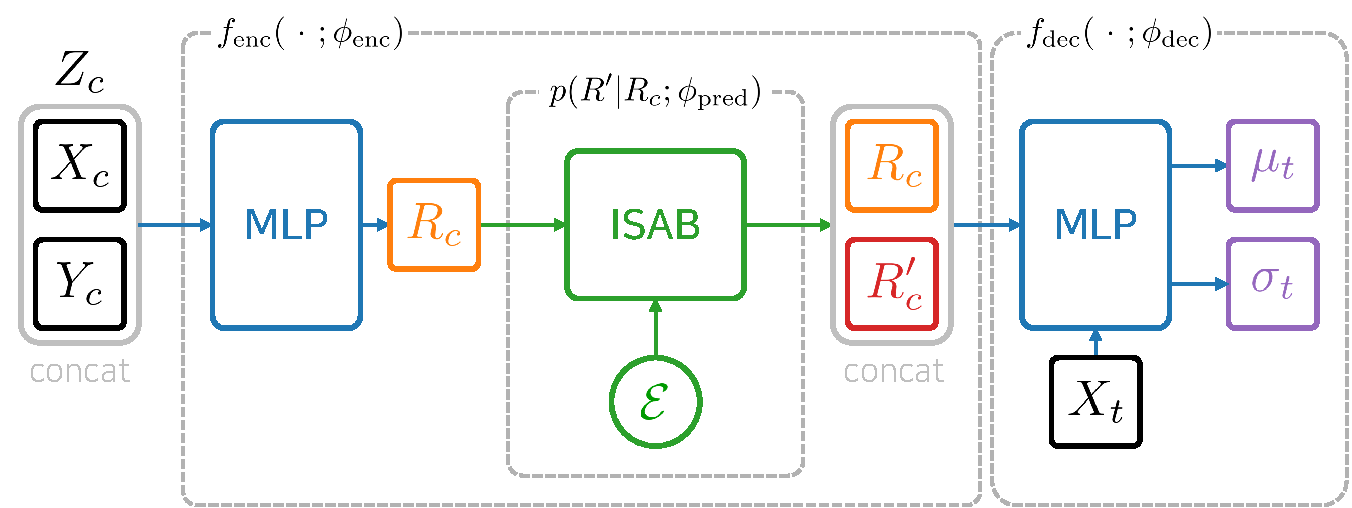
\includegraphics[width=\linewidth]{figure/main_concept.pdf}
    \caption{Concept figure of our feature generating model applied to \gls{cnp}~\citep{garnelo2018conditional}. We first convert given context dataset $Z_c$ to the representation $R_c$ using \gls{mlp} layers. Next we sample $\epsilon$ from a simple distribution (e.g. Gaussian). Then we generate the pseudo context representation $R_c'$ using generator as one layer \gls{isab}~\citep{lee2019set} in our experiment.
    %\ed{This figure is awesome!!}}
    }
    \label{figure/main_concept_mpnp}
\end{figure}
When $z$ is low-dimensional, it would be moderately easy to learn the joint predictives, but in practice, we often encounter problems with high-dimensional $z$, for instance when the input $x$ is a high-resolution image. For such cases, directly generating $z$ may be harder than the original problem, severely deteriorating the overall learning procedure of \gls{mpnp}.
Instead, we propose to generate the \emph{encoded representations} of $z$. The encoders of the most of the \glspl{npf} first encode an input $z_i$ into a representation $r_i$. For the remaining of the forward pass, we only need $r_i$s instead of the original input $z$. Hence we can build a joint predictives $p(R'|R_c; \phi_\text{pred})$ generating $R' = \{r_i'\}_{i=1}^{N-|c|}$ conditioned on $R_c = \{r_i\}_{i\in c}$ as for generating $Z'$ from $Z_c$. In the experiments, we compare these two versions of \glspl{mpnp} (generating $Z'$ and generating $R'$), and found that the one generating $R'$ works much better both in terms of data efficiency in training and predictive performances, even when the dimension of $z$ is not particularly large.
See \cref{figure/main_concept_mpnp} for our method applying to \gls{cnp} model~\citep{garnelo2018conditional}.

%%%%%%%%%%%%%%%%%%%%%%%%%%%%%%%%%%%%%%%%%%%%%%%%%%
\subsection{Training}\label{main:subsec:training}

With the generator $p(Z'|Z_c;\phi_\text{pred})$, the marginal likelihood for a task $\tau = (Z, c)$ is computed as
\[\label{eq:logmarginal_mp}
\log p(Y|X, Z_c) = \log\int \exp\bigg(-\sum_{i\in [n]}\ell(z_i, \tilde\theta(Z_c\cup Z'))\bigg) p(Z'|Z_c;\phi_\text{pred}) \dee Z'.
\]
Note that $p(Z'|Z_c;\phi_{\text{pred}})$ is \gls{cid}, so there exists a corresponding martingale posterior $\pi_N$ such that
\[
\log p(Y|X, Z_c) = \log\int \exp\bigg(-\sum_{i\in [n]}\ell(z_i, \theta)\bigg) \pi_N(\theta|Z_c) \dee \theta.
\]
We approximate the marginal likelihood via a consistent estimator,
\[\label{eq:mpnp_term1}
\log p(Y|X, Z_c) \approx \log \Bigg[ \frac{1}{K} \sum_{k=1}^K \exp\bigg(-\sum_{i\in [n]}\ell(z_i, \tilde\theta(Z_c\cup Z'^{(k)}))\bigg)
\Bigg] := -\calL_\text{marg}(\tau,\phi),
\]
where $Z'^{(1)},\dots, Z'^{(K)}\iidsim p(Z'|Z_c;\phi_\text{pred})$. This objective would be suffice if we are given sufficiently good $\tilde\theta(Z_c \cup Z'^{(k)})$, but we have to also train the encoder to properly amortize the parameter construction process \cref{eq:recovering_theta}. For this, we use only the given context data to optimize
\[\label{eq:mpnp_term2}
\log p_{\textsc{cnp}}(Y|X, Z_c) = -\sum_{i\in [n]} \ell(z_i, \tilde\theta(Z_c)) := -\calL_\text{amort}(\tau,\phi)
\]
that is, we train the parameters $(\phi_\text{enc}, \phi_\text{dec})$ using \gls{cnp} objective. Furthermore, we found that if we just maximize \cref{eq:mpnp_term1} and \cref{eq:mpnp_term2}, the model can cheat by ignoring the generated pseudo contexts and use only the original context to build function estimates. To prevent this, we further maximize the similar \gls{cnp} objectives for each generated pseudo context to encourage the model to actually make use of the generated contexts.
%\ljh{I'm not sure whether this justifies using avg outside the log rather than the avg inside the log.} 
\[\label{eq:mpnp_term3}
\frac{1}{K}\sum_{k=1}^K \log p_{\textsc{cnp}} (Y|X, Z'^{(k)}) = -\frac{1}{K}\sum_{i\in [n]} \ell(z_i, \tilde\theta(Z'^{(k)})) := -\calL_\text{pseudo}(\tau,\phi)
\]
Combining these, the loss function for the \gls{mpnp} is then
\[\label{eq:mpnp_term_whole}
\bbE_{\tau}[\calL(\tau,\phi)] = \bbE_\tau[\calL_\text{marg}(\tau,\phi) + \calL_\text{amort}(\tau,\phi) + \calL_\text{pseudo}(\tau,\phi)].
\]

% \lhg{I submitted our paper to Openreview. You can check that.}
% \ed{Thank you!!}

% \glspl{mpnp} model contains generator function $f_{\gen}$ which generates a pseudo context dataset $Z'$ or a feature of pseudo context dataset $R'$.
% To make a generator of \gls{mpnp} to sample meaningful $Z'$ or $R'$, we need to carefully construct training objective function. Otherwise, the generator tends to sample pseudo context dataset far from context dataset or collapse to one-point which does not have enough meaning or affection to target dataset. We maximize our training objective function which consists of the following terms:
% \begin{align}
%     \sum_{i=1}^n\left(\log p(y_i|x_i,Z_c,\varnothing)+\log \frac{1}{K}\sum_{k=1}^K p(y_i|x_i,Z_c,Z'^{(k)})+\frac{1}{K}\sum_{k=1}^K \log p(y_i|x_i, \varnothing, Z'^{(k)})\right)
% \end{align}
% % \ed{Thanks for updating, much clearer now. Should the third term be $p(y_i \mid x_i, \varnothing, Z'^{(k)})$ then?}
% % \lhg{Yes, that's right. We don't use context data in the third term.}\ed{I added it, hope it's ok!}
% where $K$ is the number of different generated pseudo context dataset.
% Here the first term $\log p(y|x,Z_c, \varnothing)$ implies that our amortized model should also well predict the posterior distribution of $Z$ only with context dataset. 
% The second term implies that the ensemble of our model should well predict the posterior distribution of $Z$ with context dataset and pseudo context dataset.
% The third term implies that our model should generate pseudo context dataset which well explains $Z$.
% This third term makes our model to actually generate more meaningful pseudo context dataset. 
% See \cref{app:sec:ablation_study} for generated pseudo context samples without third loss term.


% \ed{For the third term in (14), would it perhaps make more sense to put the sum inside the log, that is
% $$\log \frac{1}{K} \sum_{k=1}^K p(y_i \mid x_i, \varnothing, Z'^{(k)})$$
% so it is still kind of a posterior predictive density? Will this affect the results much?}\\
% \lhg{We empirical check that $\log \frac{1}{K} \sum_{k=1}^K p(y_i \mid x_i, \varnothing, Z'^{(k)})$ decrease the performances, and defeat by some baselines. And when I tried $\frac{1}{K} \sum_{k=1}^K \log p(y_i \mid x_i, \varnothing, Z'^{(k)})$, somewhat I think was each generated pseudo context set $Z'^{(k)}$ sampled independently and each sample should be sampled meaningfully. I mean if we use $\log \frac{1}{K} \sum_{k=1}^K p(y_i \mid x_i, \varnothing, Z'^{(k)})$, then the generator does not sample each pseudo context dataset meaningfully.}

% \lhg{
% \begin{align}
%     \log \Big(\frac{1}{K}\sum_{k=1}^K \exp{\big(\sum_{i=1}^n \log p(y_i|x_i,Z_c,Z'^{(k)})\big)}\Big) +\sum_{i=1}^n\left(\frac{1}{K}\sum_{k=1}^K \log p(y_i|x_i, \varnothing, Z'^{(k)}) + \log p(y_i|x_i,Z_c,\varnothing)\right)
% \end{align}
% }
% where $K$ is the number of different generated pseudo context dataset. Here, the first term is our posterior predictive density on $Z$, integrating over the posterior distribution of $\theta$ induced by the generator $p(Z_c' \mid Z_c)$.
% The second term  ensures our generator generates meaningful pseudo context dataset which allow the decoder to predict well.  As we are unable to evaluate the marginal likelihood $Z_c$ due to the implicit generative model, we rely on the decoder likelihood to improve the quality of $Z_c'$ samples. \lhg{For this term, we use $\frac{1}{K}\sum_{k=1}^K \log p(y_i|x_i, \varnothing, Z'^{(k)})$ instead of $\log\frac{1}{K}\sum_{k=1}^K  p(y_i|x_i, \varnothing, Z'^{(k)})$ to ensure that our generator samples each $Z'^{(k)}$s independently which well explains $Z$.} See \cref{app:sec:ablation_study} for generated pseudo context samples without this second loss term. The final term $\log p(y|x,Z_c, \varnothing)$ ensures that our amortized model also predicts well with only the context dataset. 

% \ed{Thanks for the explanation on log sum vs sum log - we should add a sentence to justify this. It looks a bit like the first term in the ELBO in equation (7). For the other point, I would prefer to leave in $\varnothing$, since the term $p(y_i \mid x_i,Z_c)$ is ambiguous, as it could be $p(y_i \mid x_i,Z_c, \varnothing)$ or $\int p(y_i \mid x_i,Z_c, Z_c') \, dp(Z_c' \mid Z_c)$. Please correct me if I'm wrong!}

% \lhg{Okay, that will be great. I added some explanations:) I have a Ph.D. admission interview next Tuesday at 16:30 KST so can we keep discussing by e-mail or comments? I understand that martingale posterior distribution is an open problem for model-data mismatch situations, is it correct?}

% \ed{Yes that's no problem, best of luck with the interview! :) @Juho should we cancel the Tuesday meeting then? We can communicate by email. Yep, model misspecification is still an open problem in the martingale posterior framework.}
% \lhg{Okay, great.}
% \ljh{No problem with me either!}

% \ed{The first term in the objective is more like the point-wise log posterior predictive density averaged over the $n$ data points, which is the KL divergence between the empirical distribution of $\mathcal{D}$ and the posterior predictive $p(y \mid x,Z_c)$.}

% \lhg{We changed our objective function. The first term changed from $\sum_{i=1}^n \log \frac{1}{K}\sum_{k=1}^K p(y_i|x_i,Z_c,Z'^{(k)})$ to $\log \Big(\frac{1}{K}\sum_{k=1}^K \exp{\big(\sum_{i=1}^n \log p(y_i|x_i,Z_c,Z'^{(k)})\big)}\Big)$.}

% \ed{
% % Nice!! And this work well? The objective is looking much better motivated now :) 
% % For the third term, we previously tried putting the avg inside the log, that is
% % $$\sum_{i \in [n]} \log \frac{1}{K} \sum_{k =1}^K  \exp\left(-\ell(z_i, \tilde\theta(Z'^{(k)}))\right),$$ and it didn't work well right? 
% Following the recent change to $\mathcal{L}_{\text{marg}}$, what about 
% $$
%  -\mathcal{L}_{\text{pseudo}}^*(\phi) =  \log \frac{1}{K} \sum_{k =1}^K  \exp\left(-\sum_{i \in [n]} \ell(z_i, \tilde\theta(Z'^{(k)}))\right),
% $$
% which is basically the first term, so a marginal likelihood, but only using $Z'^{(k)}$. The current $-\mathcal{L}_{\text{pseudo}}$ is a just lower bound on $-\mathcal{L}_{\text{pseudo}}^*$ from Jensen's inequality. 
% %Because of this, I'm guessing the results will be similar. 
% The objective would be nice and symmetric now, since it's essentially 3 (marginal) likelihood terms, corresponding to context + pseudo, only context and only pseudo.
% % If we're short on time, we can motivate $-\mathcal{L}_{\text{pseudo}}$ as being a lower bound to $-\mathcal{L}^*_{\text{pseudo}}$, that is perhaps numerically more stable. Really sorry for giving you more work Hyungi!!
% }
% \lhg{Actually, we simultaneously tried that term in experiment with (18) and sadly it didn't work well...So we fixed (18). Maybe we can justify with lower bound or something else.}
% \ed{Ah damn, that's unfortunate. Maybe we can stick to the lower bound justification then and point to the Supplementary.}
% \lhg{Yep, that will be good. Now we are trying $\lambda\calL^*$ with additional scaling factor $\lambda\geq 1$.}
% \ed{That's a good idea, perhaps we need to balance $\mathcal{L}_{\text{pseudo}}$ with $\mathcal{L}_{\text{amort}}$?}
% \lhg{That's a good point.}
% \paragraph{Main approach}
% \glspl{np} are interested in learning a latent function $f$ such that
% \begin{align*}
%     f\sim p(f),\quad y|x,f\sim p(y|x,f)
% \end{align*}
% where $(x,y)\in \calD$.
% For instance, $f$ may be parameterized by decoder neural networks of \glspl{np}, $\mu_{\dec}(\cdot;\theta)$ and $\sigma_{\dec}(\cdot;\theta)$, such that
% \begin{align*}
%     \theta\sim p(\theta),\quad y|x,\theta\sim \calN(y|\mu_{\dec}(x;\theta),\sigma_\dec^2 (x;\theta)).
% \end{align*}
% In martingale posterior neural processes, instead of assuming a prior (either for $p(f)$ or $p(\theta)$), we directly model a conditional joint predictive distributions of pseudo context dataset as,
% \begin{align*}
%     \calD_{C'}\sim p_\phi (\calD_{C'}|\calD_C),
% \end{align*}
% where $\phi$ is a parameter of joint predictive distribution and $\calD_{C'}=\{(x_i',y_i')\}_{i=1}^{n_g}$ is a generated pseudo context dataset with number of generated pseudo context data $n_g\geq 1$.
% If $(x,y)$ is high-dimensional (such as images), we can instead consider an encoded vector $r_C=f_{\enc}(\calD_C)$ and learn the joint predictive distribution of the encoded representations as $p_\phi (r_{C'}|r_C)$. Using this predictive, we can construct an empirical predictive density as
% \begin{align*}
%     g_N(x,y) = \frac{1}{|c|+n_g}\left(\sum_{i\in c}\delta_{(x_i,y_i)} + \sum_{i=1}^{n_g}\delta_{(x_i',y_i')}\right).
% \end{align*}
% The estimate of the function parameter $\theta$ should originally be obtained as
% \begin{align*}
%     \theta(g_N):=\argmin_\theta\int \ell((x,y),\theta)g_N(dx,dy),
% \end{align*}
% where in our case we set
% \begin{align*}
%     \ell((x,y),\theta)=-\log \calN (y|\mu_{\dec}(x;\theta),\sigma_{\dec}^2(x;\theta)).
% \end{align*}
% Instead of directly solving this, we introduce an amortization network with parameter $\lambda$ such that
% \begin{align*}
%     \hat{\theta}(\calD_C\cup\calD_{C'};\lambda)\approx \theta(g_N).
% \end{align*}
% Here we can see that differently generated pseudo context dataset $\calD_{C'}^{(1)}=\{(x_i'^{(1)},y_i'^{(1)})\}_{i=1}^{n_g}$ and $\calD_{C'}^{(2)}=\{(x_i'^{(2)},y_i'^{(2)})\}_{i=1}^{n_g}$ formulate different empirical predictive densities.
% Different predictive densities also formulate different amortized $\hat{\theta}$ which models functional uncertainty without both a global latent variable and a custom prior distribution.
% If we have chosen to learn the predictive of encoded representations, we first have to learn $\hat{\theta}(\cdot;\lambda)$ using only real context representation $r_C$, and put generated representation $r_{C'}$ into the amortization network later.
% \paragraph{Directly generating pseudo context data}
% In order to construct an empirical predictive density $g_N(x,y)$, we have to sample a pseudo context dataset. 
% The most straightforward approach to generate pseudo context dataset $\calD_{C'}$ is directly generating $(x_i',y_i')$ from given context dataset $\calD_C$.
% Our first attempt to formulate generator function $f_{\gen}$ was to na\"ively use ISAB~\citep{lee2019set} module as our generator and sample whole $D_{C'}$ at once.
% We use concatenated $D_C$ as inducing points $I\in\bbR^{|C|\times 2}$ in ISAB and $g$, which is \textit{i.i.d} samples from Gaussian distribution, as input $\bx\in \bbR^{n_g\times 2}$.
% Because ISAB module satisfies permutation invariance for input dataset, we can directly sample a set $\calD_{C'}$ without break exchangeability...
% \paragraph{Generating features of pseudo context data}
% \begin{figure}[t]
%     \centering
%     \includegraphics[width = \linewidth]{figure/feature model2.pdf}
%     \caption{Concept figure of our feature generating model applied to \gls{canp}~\citep{kim2018attentive}. Here we sample $g$ from a simple distribution (e.g. Gaussian). We generate key feature $r_k'$ and value feature $r_v'$ for cross attention layer which are corresponding to pseudo context data. We use generator as one layer ISAB~\citep{lee2019set} in our experiment.}
%     \label{fig:feature model2.pdf}
% \end{figure}
% As we mentioned above paragraph, directly generating pseudo context dataset is hard task, we construct our model to sample features of pseudo context dataset.
% We first encode our $\calD_c$ into $r_c\in\bbR^{|C|\times r_\text{dim}}$ with our encoder neural network $f_{\enc}$.

% See \cref{fig:feature model2.pdf} for our method applying to \gls{canp} model~\citep{kim2018attentive}.
% \subsection{Training}
% \label{main:subsec:training}
% \glspl{mpnp} model contains generator function $f_{\gen}$ which generates a pseudo context dataset $\calD_{C'}$ or a feature of pseudo context dataset $r_{C'}$.
% To make a generator of \gls{mpnp} to sample meaningful $\calD_{C'}$ or $r_{C'}$, we need to carefully construct training objective function. Otherwise, the generator tends to sample pseudo context dataset far from context dataset or collapse to one-point which does not have enough meaning or affection to target dataset. We consist our training objective function as maximizing following terms:
% \begin{align}
%     \sum_{i=1}^n\left(\log p(y_i|x_i,\calD_C)+\log \frac{1}{K}\sum_{j=1}^K p(y_i|x_i,\calD_C,\calD_{C'}^{(j)})+\frac{1}{K}\sum_{j=1}^K \log p(y_i|x_i, \calD_{C'}^{(j)})\right)
% \end{align}
% \ed{Does the $p$ in the first term above need a subscript? So something like $p_{\text{amort}}$ or something?}

% where $K$ is the number of different generated pseudo context dataset.
% Here the first term $\log p(y|x,\calD_C)$ implies that our amortized model should also well predict the posterior distribution of $\calD$ only with context dataset. 
% The second term implies that the ensemble of our model should well predict the posterior distribution of $\calD$ with context dataset and pseudo context dataset.
% The third term implies that our model should generate pseudo context dataset which well explains $\calD$.
% This third term makes our model to actually generate more meaningful pseudo context dataset. 
% See \cref{app:sec:ablation_study} for generated pseudo context samples with and without each loss terms.



\section{Experiments}
\label{sec:experiments}
\section{Experiments}

\subsection{Communication Efficiency at Scale}\label{sect:experiments_square_cube}

Before we can meaningfully evaluate SWARM parallelism, we must verify our theoretical observations on communication efficiency. Here we run several controlled experiments that measure the GPU utilization and network usage for different model sizes, using the Transformer architecture~\citep{transformer} that has been widely adopted in various fields~\citep{lin2021survey}. To decouple the performance impact from other factors, we run these experiments on homogeneous V100 GPU nodes that serve one pipeline stage over the network with varying latency and bandwidth. We use a batch size of 1 and sequences of 512 tokens; the complete configuration is deferred to Appendix~\ref{appendix:detailed_setup}.


First, we measure how the model size affects the computation to communication ratio at 500 Mb/s network bandwidth in both directions. We consider 4 model configurations: the base configuration from the BERT paper~\citep{bert}, ``xxlarge" (``large'' with $d_{model}{=}4096$),  which is used in several recent works~\citep{albert,ernie3,deberta}, and a GPT-3-scale model with $d_{model}{=}12288$~\citep{gpt3}. We also evaluate a modified Transformer architecture (``Ours'') as defined in Section~\ref{sect:experiments_large} with $d_{model}{=}4096$, 3 layers per pipeline stage and 8-bit quantized activations. As we demonstrate in Appendix~\ref{appendix:compression}, this compression strategy can significantly reduce network usage with little effect on convergence. In the first three configurations, the model consists of 12 Transformer layers placed on 12 servers with a single GPU; in the last one, there are 4 servers, each hosting 3 layers.
Appendix~\ref{appendix:detailed_setup} contains FLOP and parameter counts of each configuration.




\begin{figure}[b]
\vspace{-14pt}
    \centering
    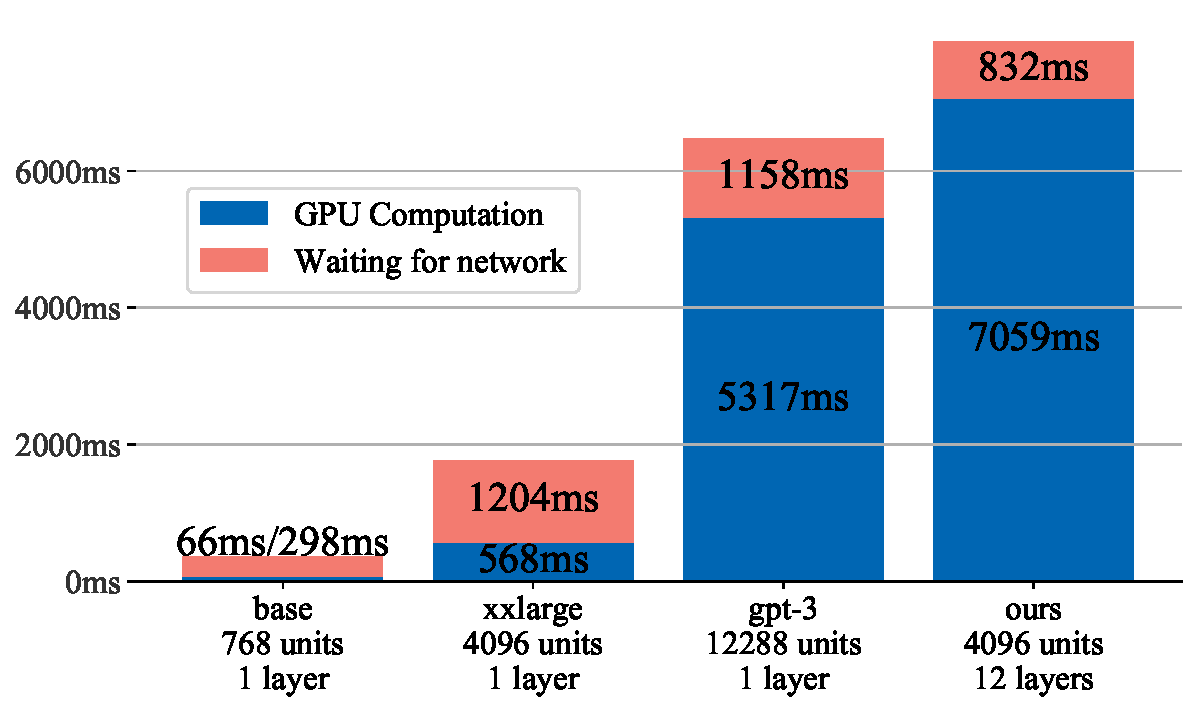
\includegraphics[width=1\linewidth]{resources/perf_absolute.pdf}
    \vspace{-12pt}
    \captionof{figure}{Pipeline computation and idle time per batch at 500 Mb/s bandwidth.}
    \label{fig:throughput_exps}
\end{figure}%
\begin{table}
    \centering
    \captionof{table}{Relative device utilization at 500 Mb/s bandwidth and varying network latency.}
    \label{tab:latency}
    \small
    \setlength{\tabcolsep}{8pt}
    \begin{tabular}[b]{@{}lcccc@{}}
    \toprule
    \multirow{2}{*}{\thead{Latency\\(RTT)}} & 
    \multicolumn{4}{c}{
    \thead{
    Relative GPU utilization\\ (100\% - idle time)
    }
    }
    
    \\
\cmidrule{2-5}                     & base & xxlarge & GPT-3 & Ours \\ \midrule
    None &   18.0\%     &  32.1\%         &  82.1\%  &  89.5\%      \\
    10ms &   11.8\%      &   28.9\%    &   79.3\%   &  87.2\%    \\
    50ms &    4.88\%      &   20.1\%    &   70.3\% &  79.5\%    \\
    100ms &    2.78\%      &    14.9\%    &  60.2\%     &   71.5\% \\
    200ms &   1.53\%     &  10.1\%    &  48.5\%   &     59.2\%    \\
    \bottomrule
    \end{tabular}
    \vspace{-6pt}
\end{table}

As depicted in Figure~\ref{fig:squarecube} (right) and Figure~\ref{fig:throughput_exps}, larger models achieve better GPU utilization rate in the same network conditions, since their communication load grows slower than computation. More importantly, even at 500 Mb/s, the resulting GPU idle time can be pushed into the 10--20\% range, either naturally for GPT-3-sized models or through activation compression for smaller models. In addition, large models maintain most of their training efficiency at the 100ms latency~(Table~\ref{tab:latency}), which is roughly equivalent to training on different continents~\citep{verizon_latency}.

\vspace{-4pt}
\subsection{Detailed Performance Comparison}\label{appendix:training_throughput}

Here we investigate how SWARM parallelism compares to existing systems for training large models: \textbf{GPipe}~\citep{huang2019gpipe} and \textbf{ZeRO-Offload}~\citep{zerooffload}.
The purpose of this section is to compare the training throughput in ``ideal'' conditions (with homogeneous reliable devices and balanced layers), as deviating from these conditions makes it \textit{infeasible} to train with baseline systems.
Still, even in such conditions the performance of different systems can vary across model architectures, and hence we want to identify the cases in which using SWARM is preferable to other approaches.
We benchmark individual SWARM components in preemptible setups in Section~\ref{sect:experiments_adaptive} and Appendix~\ref{appendix:scaling}.

We evaluate training performance for sequences of 4 Transformer layers of identical size distributed over 16 workers. Similarly to Section~\ref{sect:experiments_square_cube}, we use three layer configurations: ``xxlarge''~($d_{model} {=} 4096$, $d_{\text{FFN}} {=} 16384$, 32 heads), ``GPT-3''~($d_{model} {=} 12288$, $d_{\text{FFN}} {=} 49152$, 96 heads), and ``Ours''~($d_{model} {=} 4096$, $d_{\text{FFN}} {=} 16384$, 32 heads, 16 shared layers per block, last stage holds only the vocabulary projection layer). The microbatch size is 4 for ``xxlarge'' and 1 for ``GPT-3'' and ``Ours'', and the sequence length is 512.

To provide a more detailed view of the training performance, we measure two separate performance statistics: the training throughput and the All-Reduce time. 
The training throughput measures the rate at which the system can process training sequences, i.e., run forward and backward passes. 
More specifically, we measure the time required to process 6250 sequences of 512 tokens, which corresponds to the largest batch size used in~\citet{gpt3}.
In turn, the All-Reduce time is the time each system spends to aggregate accumulated gradients across devices. 
Intuitively, training with small batch sizes is more sensitive to the All-Reduce time (since the algorithm needs to run All-Reduce more frequently) and vice versa.


\textbf{Hardware setup:} Each worker uses a V100-PCIe GPU with 16 CPU threads (E5 v5-2660v4) and 128 GB RAM. The only exception is for ZeRO-Offload with ``GPT-3'' layers, where we had to double the RAM size because the system required 190 gigabytes at peak. Similarly to Section~\ref{sect:experiments_square_cube}, each worker can communicate at a 500 Mb/s bandwidth for both upload and download for a total of 1 Gb/s.
In terms of network latency, we consider two setups: with \textbf{no latency}, where workers communicate normally within the same rack, and with \textbf{latency}, where we introduce additional $100\pm50$ms latency directly in the kernel\footnote{More specifically, \texttt{tc qdisc add dev <...> root netem delay 100ms 50ms}}.

\textbf{GPipe configuration:} We use a popular PyTorch-based implementation of GPipe\footnote{The source code is available at \url{https://github.com/kakaobrain/torchgpipe}}. The model is partitioned into 4 stages repeated over 4 model-parallel groups. To fit into the GPU memory for the ``GPT-3'' configuration, we offload the optimizer into RAM using ZeRO-Offload. Before averaging, we use PyTorch's built-in All-Reduce to aggregate gradients.
We evaluate both the standard GPipe schedule and the 1F1B schedule~\citep{pipedream}.

\textbf{ZeRO-Offload configuration:} Each worker runs the entire model individually, then exchanges gradients with peers. For ``xxlarge'', we use the official implementation from~\cite{zerooffload}. However, for ``GPT-3'', we found that optimizer offloading still does not allow us to fit 4 layers into the GPU. For this reason, we also offload the model parameters using the \texttt{offload\_param} option.

\begin{table}
\centering
\small
\setlength{\tabcolsep}{4pt}
\captionof{table}{Training performance for different model sizes.}
\label{tab:throughput_gpt}
\begin{tabular}[b]{lcccc}
\toprule
\multirow{2}[2]{*}{System} &
  \multicolumn{2}{c}{Throughput, min/batch} &
  \multicolumn{2}{c}{All-Reduce time, min} \\ \cmidrule(lr){2-3}\cmidrule(lr){4-5} 
                 & No latency & Latency & No latency & Latency \\
 \midrule \multicolumn{5}{c}{``GPT-3'' (4 layers) }\\
 \midrule
SWARM            &  168.3 &\textbf{186.7}  &  7.4 & \textbf{7.6}   \\
GPipe            &  164.5 & 218.4 &  \multirow{2}{*}{\textbf{6.7}}    & \multirow{2}{*}{7.8}   \\
1F1B & \textbf{163.3} & 216.1 & & \\
Offload          &  272.7 & 272.7          &  25.5 & 27.3 \\
\midrule \multicolumn{5}{c}{``xxlarge'' (4 layers) }\\
\midrule
SWARM            &  44.2 & 48.2                  &  0.8  & \textbf{0.9}   \\
GPipe            &  40.1 & 108.8                  &  \multirow{2}{*}{\textbf{0.7}}  & \multirow{2}{*}{1.1}   \\
1F1B & 40.8 & 105.5 & & \\
Offload          &  \textbf{33.8} & \textbf{33.8}  &  2.8 & 4.2   \\
\midrule \multicolumn{5}{c}{Full ``Ours'' model (48 shared layers + embeddings) }\\
\midrule
SWARM            &  432.2 & 452.9                  &  0.8  &\bf 1.0   \\
GPipe            &  420.0 & 602.1                   &  \multirow{2}{*}{\bf 0.7}  & \multirow{2}{*}{1.1}   \\
1F1B             &  408.5 & 569.2 & & \\
Offload          &  \bf 372.0 &\bf 372.0  &  3.2 & 4.8   \\
\bottomrule
\end{tabular}
\vspace{-8pt}
\end{table}%

\begin{figure}[b]
\vspace{-16pt}
\centering
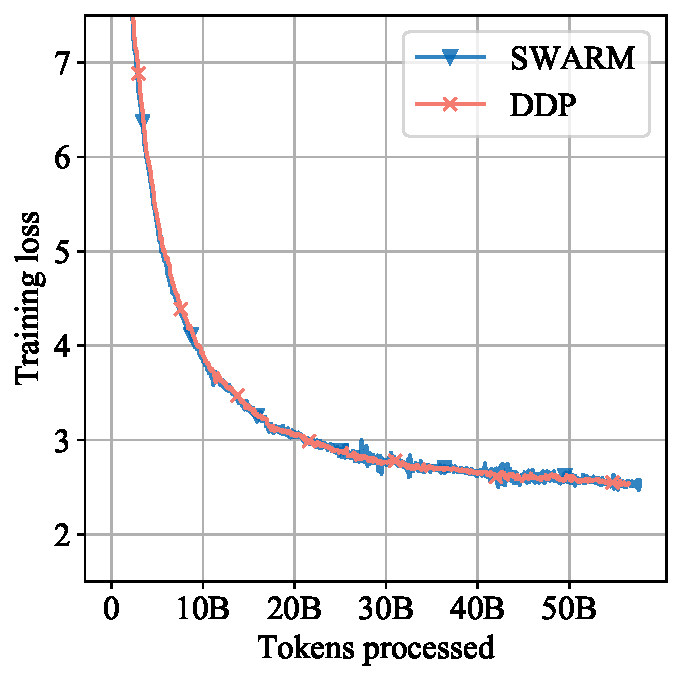
\includegraphics[ width=0.65\linewidth]{resources/learning_3stages.pdf}
\vspace{-6pt}
\captionof{figure}{Training convergence comparison.}
\label{fig:convergence}
\end{figure}

In turn, when training smaller models, ZeRO-Offload outperforms both SWARM and GPipe. This result aligns with our earlier observations in Figure~\ref{fig:squarecube}, where the same model spent most of the time waiting for the communication between pipeline stages.%

We also observe that ZeRO-Offload takes longer to aggregate gradients, likely because each peer must aggregate the entire model, whereas in SWARM and GPipe, peers aggregate a single pipeline stage. The variation between All-Reduce time in GPipe and SWARM is due to implementation differences. Overall, SWARM is competitive to HPC baselines even in an idealized homogeneous environment.

\subsection{Large-Scale Distributed Training}
\label{sect:experiments_large}

To verify the efficiency of SWARM parallelism in a practical scenario, we conduct a series of large-scale distributed experiments using preemptible (unreliable) cloud T4 and A100 GPUs over a public cloud network.

We train a Transformer language model with the architecture similar to prior work~\citep{gpt3,gptj,gptneo} and 1.01 billion parameters in total. Our model consists of 3 stages, each containing a single Transformer decoder block with $d_{model}=4096$ and 16 layers per pipeline stage. All workers within a stage serve the same group of layers, and all layers within each group use the same set of parameters, similarly to ALBERT~\citep{albert}. On top of this, the first stage also contains the embedding layer, and the last stage includes the language modeling head. Because of layer sharing, this model is equivalent to a 13B model from~\citet{gpt3} in terms of compute costs. 

We use 8-bit compression~\citep{adam8bit} for activations and gradients to reduce the communication intensity. Additional training setup details are covered in Appendix~\ref{appendix:detailed_large}.
SWARM nodes run rebalancing every $T=300$ seconds, and trainers measure peer performance using a moving average with $\alpha=0.1$. However, as we show in Section~\ref{sect:experiments_adaptive}, the throughput of SWARM is not very sensitive to the choice of these hyperparameters.



First, to verify that model parallelism with asynchronous updates does not have significant convergence issues, we train the model on the Pile~\citep{gao2020pile} dataset with 400 preemptible T4 instances, each hosting one accelerator. As a baseline, we use regular data-parallel training with offloading on 128 A100 GPUs.
We run both experiments for approximately 4 weeks and compare the learning curves.




Figure~\ref{fig:convergence} shows the results of this experiment: it can be seen that the training dynamics of two approaches are indeed similar, which demonstrates the viability of SWARM parallelism for heterogeneous and poorly-connected devices.

In the next experiment, we aim to measure the pipeline throughput in different hardware conditions and to compare it with an estimate of best-case pipeline performance.
We consider several setups: first, we use the same 400 preemptible T4 nodes; in another setup, we use 7 instances with 8 A100 GPU each; finally, we combine these fleets to create a heterogeneous setup. We examine the performance of the pipeline both with weight sharing and with standard, more common, Transformer blocks.

\begin{table}
\centering
\captionof{table}{Pipeline throughput, layer sharing.}
\label{tab:throughput}
\small
\begin{tabular}{@{}lcccc@{}}
\toprule
\multirow{2}{*}{\begin{tabular}[c]{@{}l@{}}Hardware\\ setup\end{tabular}} &
  \multicolumn{2}{c}{\begin{tabular}[c]{@{}c@{}}Throughput,\\ samples/s\end{tabular}} &
  \multicolumn{2}{c}{\begin{tabular}[c]{@{}c@{}}Optimal\\ bandwidth, Mb/s\end{tabular}} \\ \cmidrule(lr){2-3}\cmidrule(lr){4-5} 
                 & Actual & Best-case & Upload & Download \\ \midrule
T4           &  17.6      &   19.2        &   317.8     &     397.9     \\
A100          & 16.9       &   25.5        &   436.1     &     545.1     \\
T4 \& A100 &   27.3     &       ---    &   ---     &      ---    \\ \bottomrule
\end{tabular}
\end{table}
\begin{table}
\centering
\captionof{table}{Pipeline throughput, default Transformer.}
\label{tab:throughput_standard}
\small
\begin{tabular}{@{}lcc@{}}
\toprule
\multirow{2}{*}{\begin{tabular}[c]{@{}l@{}}Hardware\\ setup\end{tabular}} &
  \multicolumn{2}{c}{\begin{tabular}[c]{@{}c@{}}Throughput,\\ samples/s\end{tabular}} \\ \cmidrule(lr){2-3}
                 & Actual & Best-case \\ \midrule
T4           &  8.8      &   19.3        \\
A100          & 8.0       &   25.1        \\
T4 \& A100 &   13.4     &       ---    \\ \bottomrule
\end{tabular}
\end{table}






We measure the number of randomly generated samples processed by the pipeline both in our infrastructure and the ideal case that ignores all network-related operations (i.e., has infinite bandwidth and zero latency). The ideal case is emulated by executing a single pipeline stage 3 times locally on a single server and multiplying the single-node estimates by the number of nodes.

As demonstrated in the left two columns of Table~\ref{tab:throughput} and Table~\ref{tab:throughput_standard}, asynchronous training of compute-intensive models with 8-bit compressed activations regardless of the architecture specifics allows us to achieve high performance without a dedicated networking solution. Furthermore, the load balancing algorithm of SWARM allows us to dynamically and efficiently utilize different hardware without being bottlenecked by slower devices. 


Next, we use the same load testing scenario to estimate the bandwidth required to fully utilize each device type in the above infrastructure. For this, we measure the average incoming and outgoing bandwidth on the nodes that serve the intermediate stage of the pipeline. We summarize our findings in the right two columns of Table~\ref{tab:throughput}: it turns out that with layer sharing and 8-bit compression, medium-performance GPUs (such as T4) can be saturated even with moderate network speeds. Based on our main experiment, the optimal total bandwidth is roughly 100Mb/s higher than the values reported in Table 3 due to gradient averaging, loading state from peers, maintaining the DHT and streaming the training data.
Although training over the Internet with more efficient hardware might indeed underutilize the accelerator, this issue can be offset by advanced compression strategies such as compression-aware architectures or layer sharing, as shown in Table~\ref{tab:throughput}.

\begin{figure}[t]
    \centering
    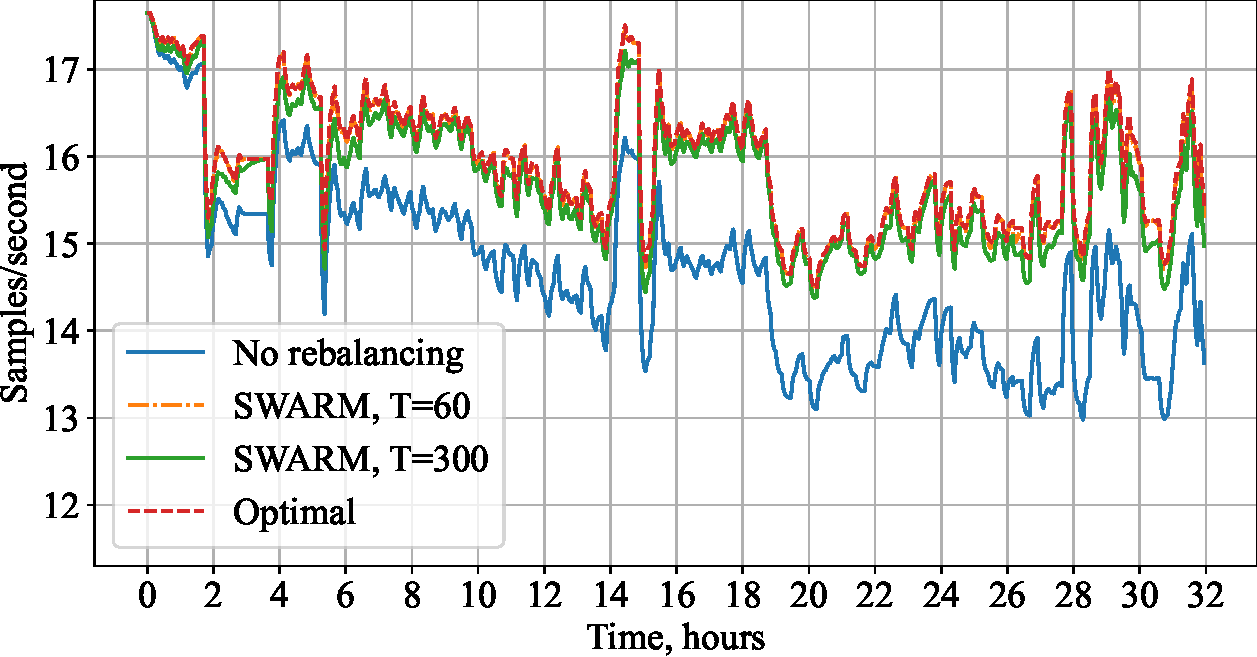
\includegraphics[width=\linewidth]{resources/rebalancing_activity.pdf}
    \captionof{figure}{Throughput of rebalancing methods over time.}
    \label{fig:rebalancing}
\end{figure}

\subsection{Adaptive Rebalancing Evaluation}


\begin{figure*}[h!]
\begin{subfigure}{0.5\textwidth}
    \centering
    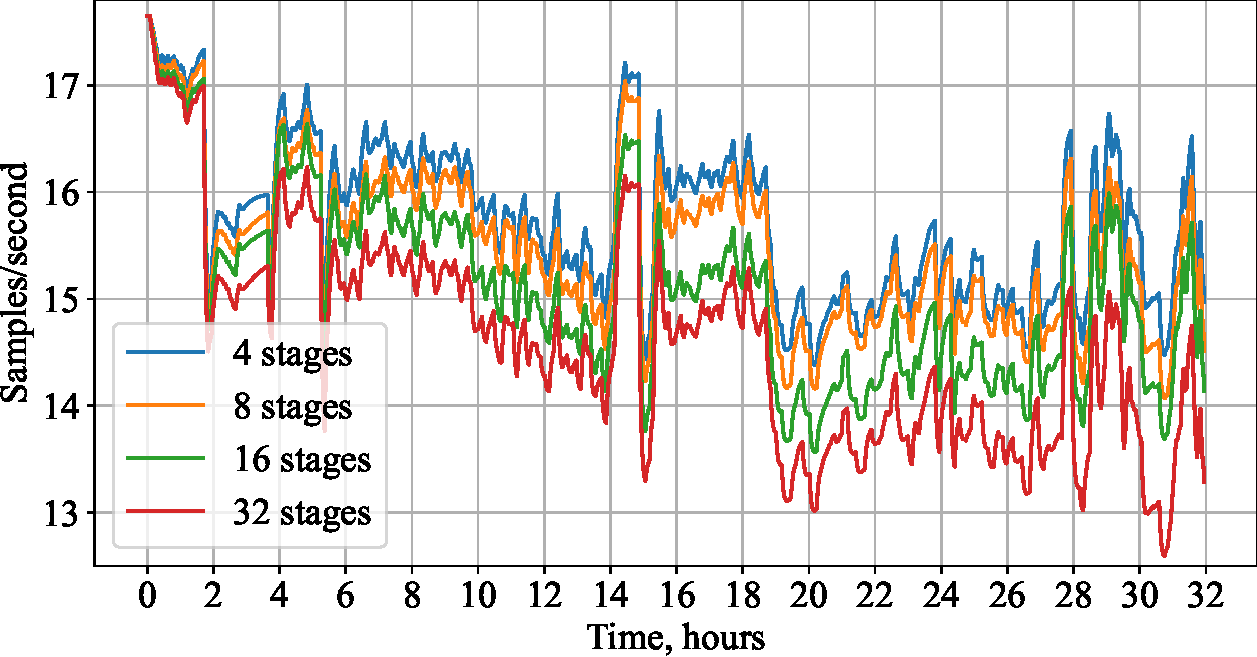
\includegraphics[width=0.97\linewidth]{resources/rebalancing_stages.pdf}
    \caption{Adaptive rebalancing of SWARM parallelism.}
    \label{fig:rebalancing_stages}
\end{subfigure}%
\begin{subfigure}{0.5\textwidth}
    \centering
    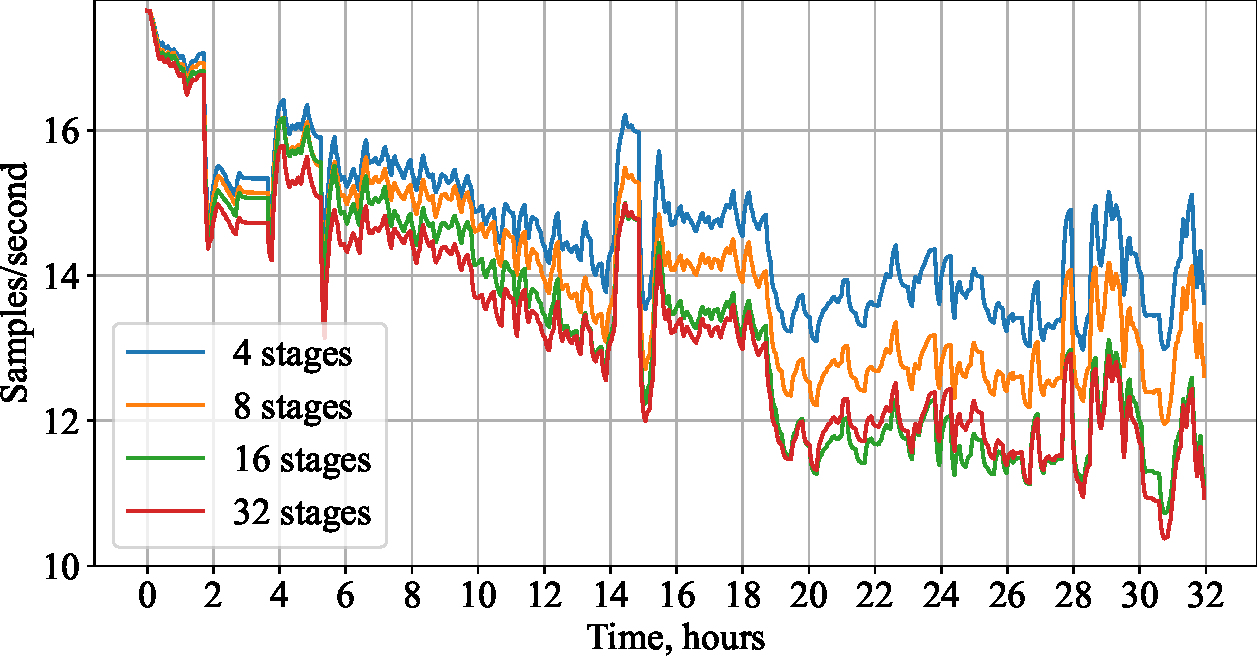
\includegraphics[width=0.97\linewidth]{resources/rebalancing_stages_baseline.pdf}
    \caption{No rebalancing.}
    \label{fig:rebalancing_stages_baseline}
\end{subfigure}
\caption{Scaling of pipeline-parallel strategies with respect to the number of stages.}
\label{fig:rebalancing_stages_all}
\end{figure*}

\label{sect:experiments_adaptive}
In this experiment, we evaluate the efficiency of adaptive peer rebalancing between stages proposed in Section~\ref{sect:method_swarm}. 
We use statistics of the number of active T4 nodes from the 32-hour segment of the experiment described in Section~\ref{sect:experiments_large}. 
We use this data to simulate training dynamics by viewing it as sequence of events, each consisting of a timestamp and a change in the number of peers (which can be positive or negative). 
When a worker is removed from the pipeline, we randomly choose the stage it was removed from: that is, removing $N$ peers corresponds to $N$ samples from the uniform distribution over four pipeline stages. 
We run 10 simulations with different random seeds and average the resulting trajectories.
We compare our strategy with two different values of $T$ to the baseline that has no rebalancing.

The results of this evaluation are available in \autoref{fig:rebalancing}; for reference, we also provide the performance of a theoretically optimal rebalancing strategy that maintains the highest possible throughput at every moment. It can be seen that even with the rebalancing period $T=300$, our approach significantly improves the overall throughput of the pipeline. When the number of peers is relatively stable, the rebalanced pipeline also approaches the optimal one in terms of throughput, which shows the efficiency of rebalancing even when moving only one node at a time.

In addition, we observed that for some brief periods, the performance of the unbalanced pipeline exceeded the throughput of the balanced one due to random choice of disconnecting peers (dropping more from the ``overrepresented'' stages affects the imbalanced pipeline less). However, this held true only for $\approx 4.5\%$ of the experiment and was quickly mitigated by adaptive rebalancing.

As expected, decreasing $T$ from 300 to 60 seconds improves both the overall throughput and the speed of convergence to optimal pipeline performance. However, the effect is not as drastic compared to the increase in DHT data transfer volume. This is also demonstrated by \autoref{tab:rebalancing_speedup}, which shows the relative throughput of the three configurations compared to the optimal one. Furthermore, the table displays that while initially there is little difference between rebalancing choices, it becomes more pronounced later on as the imbalanced version ``drifts further'' from the optimal state.

\begin{table}[b]
\centering
\captionof{table}{Relative throughput comparison of pipeline rebalancing methods.}
\small
\label{tab:rebalancing_speedup}
\begin{tabular}[b]{@{}lccc@{}}
\toprule
\multirow{2}[2]{*}{\thead{Rebalancing}} & \multicolumn{3}{c}{\% of optimal} \\ \cmidrule(l){2-4} 
                        & Overall   & First 1 hour   & Last 1 hour  \\ \midrule
None                & 82.7      & 99.0       & 45.4     \\
$T=300$    & 95.8      & 99.4       & 88.9     \\
$T=60$     & 97.6      & 99.8       & 91.7     \\ \bottomrule
\end{tabular}
\end{table}

Finally, we analyze the scaling properties of rebalancing with respect to the number of stages. To do this, we conduct experiments in the same setup as above ($T=300$) while changing the number of pipeline stages from 4 to $\{4,\ 8,\ 16,\ 32\}$. To ensure the consistency of throughput across all experiments, we increase the starting number of peers accordingly while keeping the preemption rate constant. As a baseline, we also evaluate the throughput of the pipeline that has no rebalancing.

Figure~\ref{fig:rebalancing_stages_all} shows the outcome of this experiment. As displayed in the plots, both strategies drop in performance with the increase in the stage count: while all stages should drop in performance equally in expectation, in practice, the variances are too large while the number of peers is relatively too small for the asymptotic properties to take place. This effect results in more outliers (large drops in the number of peers) in the preemption distribution for more stages. Still, rebalancing allows to partially mitigate the issue: while we observe a more consistent downward trend for the baseline strategy, the rebalanced pipeline regains its performance over time and achieves a higher overall throughput.



\section{Conclusion}
\label{sec:conclusion}
\section{Conclusion}
In this work, we advance the method of {machine unlearning} through a novel viewpoint: model sparsification, achieved by weight pruning. We show in both theory and practice that model sparsity plays a foundational and crucial role in closing the gap between exact unlearning and existing approximate unlearning methods. Inspired by that, we propose two new unlearning paradigms,  `prune first, then unlearn' and `sparsity-aware unlearn', which can significantly improve the efficacy of approximate unlearning. We demonstrate the effectiveness of our findings and proposals in extensive experiments across different unlearning setups. Our study also indicates the presence of \textit{model modularity} traits, such as weight sparsity, that could simplify the process of machine unlearning. This may open up exciting prospects for future research to investigate unlearning patterns within weight or architecture space.







% \begin{ack}
% We sincerely appreciate
% \end{ack}


\bibliographystyle{IEEEtran}
\bibliography{ref}

\newpage
\appendix

\section{Tokenizer Details}
\label{sec:tokenizer}
\subsection{Tokenizer Fertility Definition}\label{tokenizer fertility}
Fertility is defined as the average number of tokens per word \cite{acs2019}. Words are defined by the Universal Dependencies framework, which gives a "consistent annotation of grammar (parts of speech, morphological features, and syntactic dependencies) across different human languages" \cite{nivre-etal-2016-universal}. To calculate the fertility we tokenize each word from the treebank individually to get the sum total number of tokens, and then divide this by the number of words in the treebank. For Hungarian we used the test set of the "Szeged Dependency Treebank" \cite{vincze-etal-2010-hungarian}, for Thai we used the test set of the Thai "CoNLL 2017" treebank \cite{zeman-etal-2017-conll} and for English we used the test set of the "Gold Standard Universal Dependencies Corpus" \cite{silveira14gold}.

\subsection{Token Replacement Details} \label{token details}

In our work, instead of extending the tokenizer's vocabulary, we replace the least frequent tokens from it with tokens from the new language. This way, we keep the model capacity the same by controlling the vocabulary and embedding table size. 

\begin{enumerate}
\item{}Train a tokenizer limited to a vocabulary size $k$, where $k$ is the number of tokens you want to replace in the original tokenizer
\item{}Find the number of overlapping tokens $o$ between the new tokenizer of vocab size $k$, and the original tokenizer
\item{} Replace the least frequently used $k-o$ tokens from the original tokenizer with the $k-o$ tokens from the new tokenizer. Ensure that all the unchanged tokens from the original tokenizer keep the same vocabulary indices as they had before.
\begin{enumerate}
\item{}note that in the GPT2 tokenizer the tokens in the vocabulary and merges file are ordered from most frequent to least frequent, so we replace the last $k-o$ vocabulary indices in a GPT2 Tokenizer.
\end{enumerate}
\item{} The GPT2 Tokenizer executes the merges rules in the merges.txt file line by line, so to improve the efficiency on the newly added tokens, Add the merges rules from the $k-o$ new tokens to the beginning of the merges.txt file. 
\begin{enumerate}
\item{}Note that various BPE encoding algorithms are implemented without using the merges rules, so ensure that you examine your tokenizer to see how to improves the tokenizer efficiency. 
\end{enumerate}
\item{}Randomize the embeddings of the replaced tokens in the original model so the new embeddings can be learned.
\end{enumerate}

We tested this tokenizer to ensure that the encoding and decoding of text works properly, and figure \ref{fig:fertility} shows that it also improves the fertility.


\section{Base Model}
\label{base_model}
We train our base model with the same tokenizer and architecture as GPT-2 model \cite{radford2019language}. The model has 40 layers of transformer blocks with hidden dimension 5120 and 13 billion parameters in total. The vocabulary size is 50260. The base model was pretrained on 300B English tokens from the PILE\cite{gao2020pile} and C4\cite{raffel2023exploring} datasets, filtered for only natural language English text.

\section{Datasets}
\label{sec:dataset_details}
\subsection{English pretraining data} \label{english pretraining data}
For the continuous pretraining phase, we often mix English data with either Hungarian or Thai. The English data we used is a 100 gigabyte sample of data from the base model pretraining corpus introduced in section \ref{base_model}.

\subsection{English instruction tuning data} \label{english instruction tuning data}
To construct our English instruction tuning dataset, we sample each constituent task from FlanV2 \cite{longpre2023flan} and OIG \cite{Nguyen_2023} equally by raw text size with a fixed dataset size budget. This creates an instruction tuning dataset that is task diverse and reasonably sized. The benefit of sampling instruction tuning data at the task level is shown in  \cite{iyer2023optiml}, and provides a compute efficient alternative to training on all the data. The dataset is 2.6 gigabytes of raw text and about 1.9 million samples.

\subsection{Hungarian pretraining tuning data}\label{hungarian pretraining data}
The dataset used for Hungarian pretraining is the Hungarian Webcorpus 2.0 \cite{Nemeskey:2020}. Our dataset is 96 gigabytes and 11,152,900 documents.

\subsection{Hungarian instruction tuning tuning data}\label{hungarian instruction tuning data}
 There is a lack of naturally written Hungarian instruction tuning datasets, so we use google translate to translate our English Instruction tuning corpus \ref{english instruction tuning data} to Hungarian. During translation the prompt and completion are translated separately and only concatenated during training. 

\subsection{Thai pretraining data}\label{thai pretraining corpus}
For the Thai pre-training corpus, we combine the Thai subsets of OSCAR \cite{abadji2022cleaner}, MC4 \cite{xue-etal-2021-mt5}, and CCNet \cite{wenzek2019ccnet}, which are all derived from Common Crawl. The entire combined corpus was processed with MinHash deduplication \cite{chenghao_mou_2023_8364980, 666900} with 1-grams and a Jaccard similarity of 0.6, with sentence level n-grams (split by whitespace), and totals 15.32 million documents.

\subsection{Thai instruction tuning data}\label{thai instruction tuning corpus}
For Thai instruction tuning data, we use a mixture of manually templated Thai datasets, as well as existing IT datasets translated from English. 

We take various Thai NLP datasets and create a variety of prompting templates for each task to form an instruction tuning dataset. These consist of translation \cite{Nomoto2019InterpersonalMA} \cite{BuschbeckWolf2020APE} \cite{Riza2016IntroductionOT} \cite{Ladhak2020WikiLinguaAN} \cite{cettolo-etal-2012-wit3} \cite{team2022NoLL}, NLI \cite{Conneau2018XNLIEC}, QA \cite{Artetxe:etal:2019} \cite{kobkrit_viriyayudhakorn_2021_4539916}, text categorization, sentiment analysis \cite{bact_2019_3457447}, and summarization \cite{chumpolsathien_2020} \cite{hasan-etal-2021-xl} tasks. This collection of datasets totals 6.26 million instruction tuning examples.

The English-translated IT datasets consist of traditional instruction tuning, multi-turn conversation, and domain-specific QA (i.e. general knowledge, finance, science, mathematics) sourced from collections like FLAN \cite{longpre2023flan}, OIG \cite{Nguyen_2023}, Alpaca \cite{alpaca}, Dolly \cite{DatabricksBlog2023DollyV2}, HC3 \cite{guo-etal-2023-hc3}, and OpenAssistant \cite{Kopf2023OpenAssistantC}, totalling 1.06 million examples.

\section{Training Details}
\label{sec:training_details}

\subsection{Pretraining Hyperparameters}\label{pretraining hyperparameters}
The training process utilized cross-entropy loss to optimize the CLM objective. All training runs shared the same hyperparameters to ensure a fair comparison and to avoid hyperparameter searches. When comparing two pre-training ablations, the runs were trained to token parity, training on the same number of tokens regardless of available data or tokenizer efficiency

The hyperparameters used were batch size = 512, fixed learning rate = 0.000015 and weight decay = 0.1. All the tokens were packed into the training sequences, if they did not fit in a sequence then they would be placed in the next sequence so no training tokens are lost.\footnote{\label{note}\href{https://github.com/sambanova/generative_data_prep}{https://github.com/sambanova/generative\_data\_prep}} An attention mask was applied so that only tokens from the same article attend to each other.
 

\subsection{Instruction Tuning Hyperparameters}\label{instruction tuning hyperparameters}
All instruction tuning studies share the same hyper-parameters. But ablations comparing runs are not run to step parity, rather they are all trained to 1 epoch to ensure they see all the data.

The hyperparameters used are batch size = 128, fixed learning rate = 0.000015, weight decay = 0.1, grad norm clip = 1.0, and prompt loss weight = 0.0 to ensure that prompts are attended to but not trained on. All the tokens were packed into sequences in a greedy fashion, if they did not fit in a sequence then they would be discarded.\footnotemark[1] An attention mask was applied so that only tokens from the same article attend to each other.

\subsection{Hardware Configuration}\label{hardware}
All training is run on SambaNova's Reconfigurable Data Units (RDU) \cite{9567250}.

% \section{Baselines}
% \label{sec:app_ext_baselines}
% \input{texts/appendix_extended_baselines}

% \section{Model Alignment Details}
% \label{sec:app_training_details}
% \input{texts/appendix_training_details}

% \section{API Selection Complexity Score}
% \label{sec:app_complexity_metrics}
% \input{texts/appendix_3m_model}

\section{Evaluation}
\label{sec:evaluation}
The EAI evaluation harness\cite{eval-harness} is used for all benchmarking. The code\footnote{our open source eval suite link} was adapted for new tasks to evaluate the models on non-English languages. We categorize all the tasks into 4 categories:


\paragraph{Multiple-choice} In this category of tasks, we append each candidate option after the prompt and let the model pick answer with the highest probability. We report average accuracy on each tasks.

\begin{table}[!h]
\centering
\caption{Multiple Choice Evaluation Benchmarks}
\label{tab:table-label}
\begin{tabular}{|c|m{0.8\textwidth}|}
\hline
\textbf{Language} & \textbf{Evaluation Tasks} \\
\hline
English & Lambada \cite{paperno2016lambada}, HellaSwag \cite{zellers2019hellaswag}, Openbookqa \cite{mihaylov2018suit}, Boolq \cite{clark2019boolq}, Arc Easy and Challenge \cite{clark2018think}, PiQA \cite{bisk2019piqa}, ANLI R1 \cite{nie2020adversarial} and Winogrande \cite{sakaguchi2019winogrande}. \\
\hline
Hungarian & HULU evaluation suite \cite{ligetinagy2022hulu}, which is composed of human translated tasks HuCB, HuSST, HuWNLI, HuCOPA, HuCOLA and HuRTE. \\
\hline
Thai &  XCOPA \cite{ponti2020xcopa} and WiseSight Sentiment Analysis \cite{bact_2019_3457447} corpus. Translated versions of HellaSwag \cite{zellers2019hellaswag}, MultiRC \cite{MultiRC2018}, RTE \cite{wang2019superglue}. \\
\hline
% Add more rows as needed
\end{tabular}
\end{table}


\paragraph{Open-ended Question Answering} In this category of tasks, we let the model to freely generate completions for each question prompt and we report the average F1 score between the model output and the ground truth answer. 

\begin{table}[!h]
\centering
\caption{Open-ended Question Answering Evaluation Benchmarks}
\label{tab:table-label}
\begin{tabular}{|c|m{0.8\textwidth}|}
\hline
\textbf{Language} & \textbf{Evaluation Tasks} \\
\hline
Hungarian & translated versions of BoolQ \cite{clark2019boolq} and Natural Questions \cite{47761} \\
\hline
Thai &  XQuAD \cite{Artetxe:etal:2019} and a translated version of ReCoRD \cite{Zhang2018ReCoRDBT} \\
\hline
% Add more rows as needed
\end{tabular}
\end{table}







\paragraph{Summarization} In this category of tasks, we let the model freely generate a summary for each prompt and we report average ROUGE-2 score between the model output and ground truth. 

\begin{table}[!h]
\centering
\caption{Summarization Evaluation Benchmarks}
\label{tab:table-label}
\begin{tabular}{|c|m{0.8\textwidth}|}
\hline
\textbf{Language} & \textbf{Evaluation Tasks} \\
\hline
Hungarian & Translated version of XSum \cite{narayan2018dont}. \\
\hline
Thai &  ThaiSum \cite{chumpolsathien_2020} \\
\hline
% Add more rows as needed
\end{tabular}
\end{table}


\paragraph{Translation} In this category of tasks, we let the model to freely generate translated text and we report BLEU score between the model output and the ground truth answer. 

\begin{table}[!h]
% \vspace{-42pt}
\centering
\caption{Translation Evaluation Benchmarks}
\label{tab:table-label}
\begin{tabular}{|c|m{0.8\textwidth}|}
\hline
\textbf{Language} & \textbf{Evaluation Tasks} \\
\hline
Hungarian & wmt 2009 en-hu and wmt 2009 hu-en \footnote{\href{https://www.statmt.org/wmt09/}{https://www.statmt.org/wmt09/}} datasets \\
\hline
Thai & WIT3 Ted Talks Corpus \cite{cettolo-etal-2012-wit3} \\
\hline
% Add more rows as needed
\end{tabular}
\end{table}


\end{document}
